%! TeX root = master.tex
% !TEX program = lualatex

\lecture{5}{18-03-2026}{k-Nearest Neighbors and Feature Expansion}{}
\section{Non-linear Model}
\subsection{Histograms}
A histogram in $\mathbb{R}^D$ is a $D-$dimensional vector such that \[
  x^{\left(d\right)} \in [0,1], \forall 1 \leq d \leq D \quad
  \sum_{d=1}^{D}x^{\left(d\right)} = 1 
\]
Given a vector in $\mathbb{R}^D$ whose values are all non-negative(and at least one is strictly positive), 
one can obtain a histogram by dividing each value by the sum of values. 

\subsection{k-Nearest neighbor method}
We assign the label/value of the nearest neighbor. \\
For $classification$ it consists to give to similar data samples the same label, and for $regression$, the same associated value.

\subsubsection{k-NN: Algorithm}
\textbf{Classification:}
\begin{enumerate}
  \item Compute the distance between the test sample \textbf{x} and all training samples \textbf{\{$x_i$\}}
  \item Find the $k$ sample $\{ x_{NN1}, \dots, x_{NNK} \}$ with the minimum distances
  \item Find the most common label among these $k$ nearest neighbors (majority vote)
  \item Assign the corresponding label/value \textbf{y}$_{MV}$ to the test sample
\end{enumerate}
If several labels appear the same number of times among the $k$-NN, one strategy
consists of taking the one whose samples have the smallest average distance to
the test sample

\textbf{Regression:}
\begin{enumerate}
  \item Compute the distance between the test sample \textbf{x} and all training samples \textbf{\{$x_i$\}}
  \item Find the $k$ sample $\{ x_{NN1}, \dots, x_{NNK} \}$ with the minimum distances
  \item Compute the value $\hat{y}$ for the test sample based on that of these $k-$NN
\end{enumerate}

\subsubsection{k-NN: Properties}
\begin{itemize}
  \item The results may change for different distance functions. (assigning to a different class)
  \item The $k$-NN \textbf{doesn't train a model} (no learning), it only keep the data from the training, and use them to predict the label for the test data. 
So we need: good data representation, a distance function and a given value $k$ \to the results \textbf{depends} on the value $k$. 
  \item This is refered to as a \textbf{non-parametric} learning method (no parameters to optimize during training) and $k$ is said to be a $hyper-parameter$, set manually.
  
  So we need: good data representation, a distance function and a given value $k$ \to the results \textbf{depends} on the value $k$. 
\item The features have to be \textbf{normalized} to compute the distance (all features have the same weight).
  \item It is \textbf{computationally expensive} as for each test sample, we need to compute the distances to all training samples. To avoid this problem 
  we could approximate the nearest neighbor by using: Hashing or kd-trees.
\item \textbf{Curse of dimensionality}, in the real world data tends to be very high dimensional (ex: for an image of 536 x 356 in 3D $x_i \in \mathbb{R}^{536 \cdot 356 \cdot 3}$), in such dimension, all points tend to be far apart. 
\end{itemize}

\subsection{Feature expansion}
To handle some non linear data, we could use a polynomial curve that transform the input and separate our classes. 

And then we can apply a linear model to the resulting variable to find the decision boundary :
i.e :

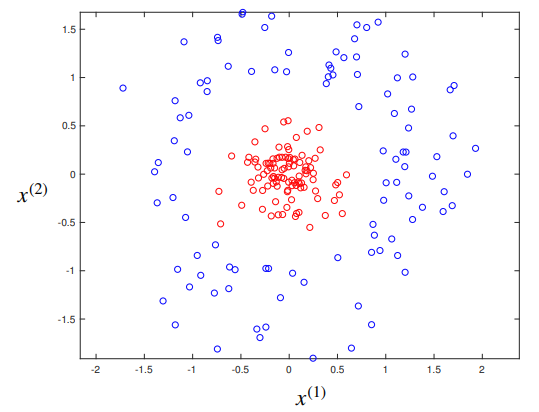
\includegraphics[width=0.3\linewidth]{images/img_20260318_163111.png}
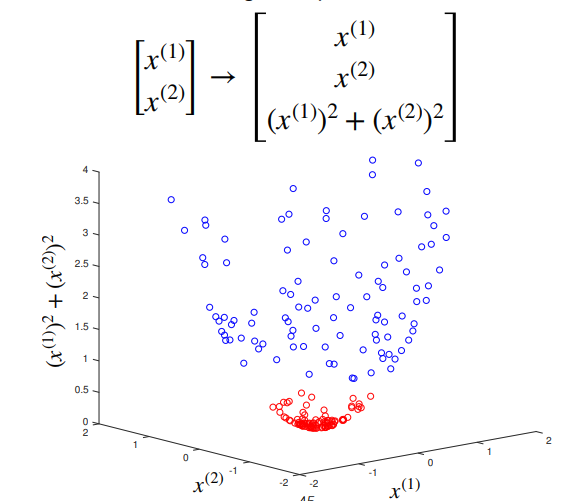
\includegraphics[width=0.3\linewidth]{images/img_20260318_163124.png}
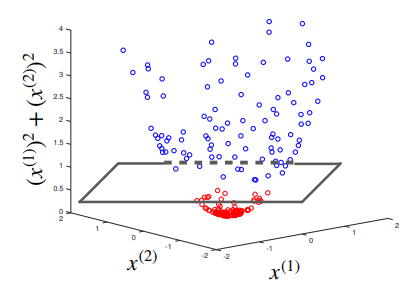
\includegraphics[width=0.3\linewidth]{images/img_20260318_163348.png}


\begin{wrapfigure}{r}{0.2\linewidth}
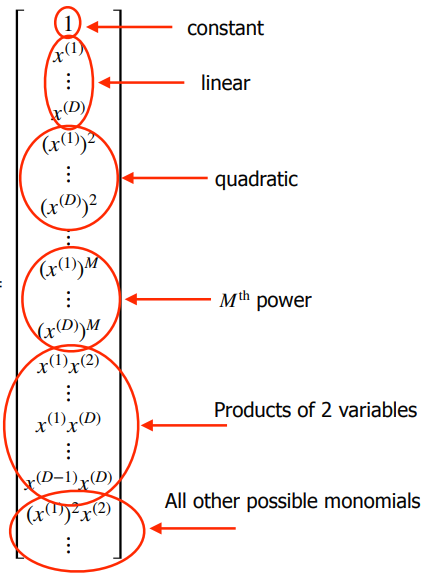
\includegraphics[width=\linewidth]{images/img_20260318_164148.png}
\end{wrapfigure}

So this consists, of performing a \textbf{change of variable} $x \to \phi (x)$. 

In general for $D-$ dimensional inputs, we can obtain a large $\phi(x)$ 

\phi(x) is found by mapping the samples from different classes in two different direction. 

I.e 
\[
  class 1: \left|x\right| < 1.2 \quad class 2: \left|x\right| > 2.0 
  
  \text{Then :} x^2 - 1.44 \leq \phi(x) \leq x^2 - 4 
\]

The resulting expanded features can then be used in any linear alogrithm that we have seen previously.

As the polynomial feature expansion uses a mapping from $x \in R^D$ to another representation $\phi(x) \in \mathbb{R}^F$, where $
F \gg D$, we can use a linear model in this new space and write \[
  \hat{y}_i = w^T \phi(x_i)
\]where now $w \in \mathbb{R}^F$. 

To use it with linear regresion, we rewrite the least-square loss like this \[
  min_w \sum_{i=1}^{N}(w^T \phi(x_i) - y_i)^2 \quad w \in \mathbb{R}^F \text{(not $\mathbb{R}^{D+1}$ anymore)}  
\]

This new function is still convex, and its gradient is given by: \[
  \nabla R = 2 \sum_{i=1}^{N}\phi(x_i)^T w - y_i) 
\] 
Setting it to zero we get a $F \times F \cdot F \times 1$ matrix
\[
\left(\sum_{i=1}^{N}\phi(x_i)\phi(x_i)^T \right)w^* = \sum_{i=1}^{N}\phi(x_i)y_i 
\]

Then we group the transformed inputs $\{\phi(x_i)\}$ and the outputs $\y_i\}$ in a matrix vector of the form \[
  \phi = \begin{pmatrix}
     \phi(x_1)^T  \\
     \vdots \\
     \phi(x_N)^T 
   \end{pmatrix} \in \mathbb{R}^{N \times F}
y = \begin{pmatrix}
   y_1  \\
   \vdots \\ y_N  
\end{pmatrix} \in \mathbb{R}^N
 \] 
 Then, we have  \[
   w^* = (\phi ^T \phi)^{-1}\phi ^T y
 \]

 \subsubsection{Mapping to a higher-dimensional sapce}
 We can observe, that the mapping $\phi(\cdot)$ always increases the dimension of the input. We do this because increasing the dimensionality allows linear models to represent nonlinear relationships, but only if the feature mapping is nonlinear. 

 \subsubsection{Feature expansion: Properties}
 It is an effective way to use linear model on non linear data samples, but it requires choosing the degree of the polynomial. 
 
 In fact, we could use \textbf{any} function on the input (not only polynomials !!). 
 
